% -------------------------------------------------------------------------------------------------
%      MDSG Latex Framework
%      ============================================================================================
%      File:                  introduction-[UTF8,ISO8859-1].tex
%      Author(s):             Michael Duerr
%      Version:               1
%      Creation Date:         30. Mai 2010
%      Creation Date:         30. Mai 2010
%
%      Notes:                 - Example chapter
% -------------------------------------------------------------------------------------------------
%
\chapter{Related Work}\label{sec:RelatedWork}
- Definition of field of research \\
- Scientific Scope \\
- Which comparable work in research exists? \\
- Separation from other works

\section{Reinforcement learning}
%https://lilianweng.github.io/lil-log/2018/02/19/a-long-peek-into-reinforcement-learning.html#key-concepts
\marginpar{rl components}
Reinforcement learning (RL) in its core is defined by Sutton and Barto as ``learning from 
interaction to achieve a goal'' \cite{suba18}. As displayed in Figure \ref{fig:rl_cycle}
the authors divided the  consists of the following components: an environment,
one or multiple agents and time sensitive information like environment states $S_{t}$,
agent actions $A_{t}$ and rewards $R_{t}$.
\begin{figure}[hpbt]
    \centering
    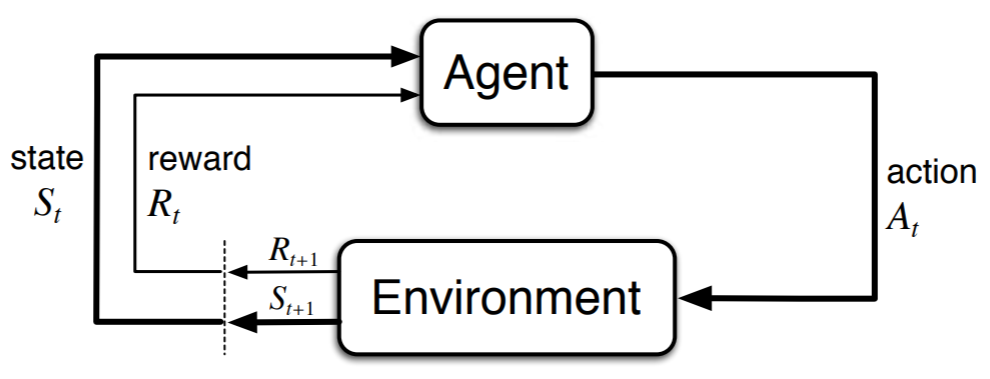
\includegraphics[width=0.6\textwidth]{pictures/RLInteractionSB}\\
    \caption[reinforcement learning cycle]{The cycle of agent-environment interaction as shown in ``Reinforcement learning: An introduction''\cite{suba18}}\label{fig:rl_cycle}
\end{figure}

\marginpar{learning}
Initially an agent has no knowledge of good or bad actions and learns as it acts in an
environment. Based on the executed action the environment changes and returns the new
state $s'_{t}$ and a reward back to the agent. The agent processes those environment
signals and chooses the next action with the goal of maximizing the rewards. Hence
RL is a cycle which ends once a condition is reached.

\marginpar{policy}
Sutton and Barto, the authors of ``Reinforcement learning: An introduction'' \cite{suba18},
define the agents action selection with respect to the current state as a policy $\pi$.
They explain further that a policy could be as simple as a lookup table, mapping
states to actions or it could contain a complicated search process for the best
decision. In most cases it is of stochastic nature, mapping actions and states with
probabilities. During environment interactions agents gain rewards, which then can be
used to update the policy accordingly. For example, should the reward, which is a number,
be low or even negative it could be interpreted as a penalty. In return the policy
could then be adapted to set a very low probability for that action in combination with
that certain state. So next time the agent finds itself in that state the bad action is
not very likely to be chosen again.

\marginpar{value function}
While rewards only rate the immediate situation, a value function $v(s)$ can be
used to estimate the long term value of a state. The resulting value is the total reward
an agent could get down the line,
starting from a state $s$. This is of importance, since an action
could result in a new state with high reward but afterwards could lie a low reward
streak. Or the opposite could be the case, where an action resulting in a low reward
could subsequently yield high rewards. Sutton and Barto claim, that the reward estimation
is a key function of RL, since the goal is to achieve as much reward as possible.

\marginpar{exploration vs exploitation}
The last part to note about RL is that it entails the problem of balancing
exploration and exploitation. In order to learn, an agent has to explore the options
given. However, since the highest reward is the goal an agent could become greedy
and always choose actions of which is known to result in reward. If an agent doesn't
explore enough the best strategy will stay hidden and if an agent always explores
without exploiting the gained knowledge chances are that the reward will not be as good.

\section{Credit assignment problem}
\marginpar{intro (single and multi)}

\marginpar{intro}
RL in the real world often involves multiple agents solving problems together, for
example working in warehouses and factories. In this case agents apply actions in a shared
environment and try to work together to reach a goal. However, for each multi-action sequence
the environment only returns one global reward.   The environment only returns one
global reward to be shared by all agents.
and execute actions
simultaneously.  consists of a shared environment between multiple agents. An example
is
stocking warehouses or playing against each other in multiplayer games. However
having one environment containing multiple agents also comes with great difficulties for
the learning process.     can be conducted in a multi-agent environment, there are a few difficulties
that needs to be faced.
\marginpar{CAP example}
\marginpar{CAP and diff kinds}

\section{Markets}
\marginpar{markets and advantage}
\marginpar{sm}
\marginpar{am}
\marginpar{what is expected?}

